% # 4.2 使用future

假设你要乘飞机去国外度假,当到达机场办理完各种登机手续后,还需要等待机场广播通知登机。这段时间内,你可能会在候机室里面找一些事情来打发时间,比如:读书,上网,或者来一杯咖啡。不过,你就在等待一件事情:机场广播通知登机。

C++标准库将这种事件称为future。当线程需要等待特定事件时,某种程度上来说就需要知道期望的结果。之后,线程会周期性(较短的周期)的等待或检查事件是否触发(检查信息板),检查期间也会执行其他任务(品尝昂贵的咖啡)。另外,等待任务期间也可以先执行另外的任务,直到对应的任务触发,而后等待future的状态会变为就绪状态。future可能是和数据相关(比如,登机口编号),也可能不是。当事件发生时(状态为就绪),这个future就不能重置了。

C++标准库中有两种future,声明在\texttt{<future>}头文件中: unique future(\texttt{std::future<>})和shared futures(\texttt{std::shared\_future<>}),与了\texttt{std::unique\_ptr}和\texttt{std::shared\_ptr}非常类似。\texttt{std::future}只能与指定事件相关联,而\texttt{std::shared\_future}就能关联多个事件。后者的实现中,所有实例会在同时变为就绪状态,并且可以访问与事件相关的数据。这种关联与模板有关,比如\texttt{std::unique\_ptr} 和\texttt{std::shared\_ptr}的模板参数就是相关的数据类型。与数据无关处的,可以使用\texttt{std::future<void>}与\texttt{std::shared\_future<void>}的特化模板。虽然,我倾向于线程通讯,但future对象本身并不提供同步访问。当多个线程需要访问一个独立future对象时,必须使用互斥量或类似同步机制进行保护。不过,当多个线程对一个\texttt{std::shared\_future<>}副本进行访问,即使同一个异步结果,也不需要同步future。

并行技术规范将这两个模板类在\texttt{std::experimental}命名空间中进行了扩展:\texttt{std::experimental::future<>}和\texttt{std::experimental::shared\_future<> }。这个命名空间是为了将其与\texttt{std}命名空间中的模板类进行区分,实验命名空间中为这两个模板类添加了更多的功能。尤其是\texttt{std::experimental}中的内容与代码质量无关(我希望这里也会有较高质量的实现),需要强调的是这个命名空间提供的都不是标准类和函数,这个命名空间中类和函数的语法和语义,很可能与纳入C++标准(也就是\texttt{std}命名空间)后有所不同。如果想要使用这两个试验性的模板类,需要包含\texttt{<experimental/future>}头文件。

最简单的事件,就是在后台运行的计算操作。第2章中已经清楚了\texttt{std::thread} 执行的任务不能有返回值,不过这个问题能使用future进行解决。

\mySubsubsection{4.2.1}{后台任务的返回值}

假设有一个需要长时间的运算,需要计算出一个有效值,但并不迫切需要这个值。你可以启动新线程来执行这个计算,你需要计算的结果,而\texttt{std::thread}并不提供直接接收返回值的机制。这里就需要\texttt{std::async}函数模板(也是在头文件`<future>`)。

当不着急让任务结果时,可以使用\texttt{std::async}启动一个异步任务。与\texttt{std::thread}对象等待的方式不同,\texttt{std::async}会返回一个\texttt{std::future}对象,这个对象持有最终计算出来的结果。当需要这个值时,只需要调用这个对象的get()成员函数,就会阻塞线程直到future为就绪为止,并返回计算结果。

代码4.6 \texttt{std::future}从异步任务中获取返回值

\begin{cpp}
#include <future>
#include <iostream>

int find_the_answer_to_ltuae();
void do_other_stuff();
int main()
{
  std::future<int> the_answer=std::async(find_the_answer_to_ltuae);
  do_other_stuff();
  std::cout<<"The answer is "<<the_answer.get()<<std::endl;
}
\end{cpp}

与\texttt{std::thread}方式一样,\texttt{std::async}允许通过添加额外的调用参数,向函数传递额外的参数。第一个参数是指向成员函数的指针,第二个参数提供这个函数成员类的具体对象(是通过指针,也可以包装在\texttt{std::ref}中),剩余的参数可作为函数的参数传入。否则,第二个和随后的参数将作为函数的参数,或作为指定可调用对象的第一个参数。和\texttt{std::thread}一样,当参数为右值时,拷贝操作将使用移动的方式转移原始数据,就可以使用“只移动”类型作为函数对象和参数。

代码4.7 使用\texttt{std::async}向函数传递参数

\begin{cpp}
#include <string>
#include <future>
struct X
{
  void foo(int,std::string const&);
  std::string bar(std::string const&);
};
X x;
auto f1=std::async(&X::foo,&x,42,"hello");  // 调用p->foo(42, "hello"),p是指向x的指针
auto f2=std::async(&X::bar,x,"goodbye");  // 调用tmpx.bar("goodbye"), tmpx是x的拷贝副本
struct Y
{
  double operator()(double);
};
Y y;
auto f3=std::async(Y(),3.141);  // 调用tmpy(3.141),tmpy通过Y的移动构造函数得到
auto f4=std::async(std::ref(y),2.718);  // 调用y(2.718)
X baz(X&);
std::async(baz,std::ref(x));  // 调用baz(x)
class move_only
{
public:
  move_only();
  move_only(move_only&&)
  move_only(move_only const&) = delete;
  move_only& operator=(move_only&&);
  move_only& operator=(move_only const&) = delete;

  void operator()();
};
auto f5=std::async(move_only());  // 调用tmp(),tmp是通过std::move(move_only())构造得到
\end{cpp}

future的等待取决于\texttt{std::async}是否启动一个线程,或是否有任务在进行同步。大多数情况下,也可以在函数调用之前向\texttt{std::async}传递一个额外参数,这个参数的类型是\texttt{std::launch},还可以是\texttt{std::launch::defered},表明函数调用延迟到wait()或get()函数调用时才执行,\texttt{std::launch::async}表明函数必须在其所在的独立线程上执行,\texttt{std::launch::deferred | std::launch::async}表明实现可以选择这两种方式的一种。最后一个选项是默认的,当函数调用延迟,就可能不会再运行了。如下所示:

\begin{cpp}
auto f6=std::async(std::launch::async,Y(),1.2);  // 在新线程上执行
auto f7=std::async(std::launch::deferred,baz,std::ref(x));  // 在wait()或get()调用时执行
auto f8=std::async(
              std::launch::deferred | std::launch::async,
              baz,std::ref(x));  // 实现选择执行方式
auto f9=std::async(baz,std::ref(x));
f7.wait();  //  调用延迟函数
\end{cpp}

本章的后续小节和第8章中,会再次看到这段程序,使用\texttt{std::async}会将算法分割到各个任务中,这样程序就能并发了。不过,这不是让\texttt{std::future}与任务实例相关联的唯一方式,也可以将任务包装入\texttt{std::packaged\_task<>}中,或通过编写代码的方式,使用\texttt{std::promise<>}模板显式设置值。与\texttt{std::promise<>}相比,\texttt{std::packaged\_task<>}具有更高的抽象,所以我们从“高抽象”模板说起。

\mySubsubsection{4.2.2}{future与任务关联}

\texttt{std::packaged\_task<>}会将future与函数或可调用对象进行绑定。当调用\texttt{std::packaged\_task<>}对象时,就会调用相关函数或可调用对象,当future状态为就绪时,会存储返回值。这可以用在构建线程池(可见第9章)或其他任务的管理中,比如:在任务所在线程上运行其他任务,或将它们串行运行在一个特殊的后台线程上。当粒度较大的操作被分解为独立的子任务时,每个子任务都可以包含在\texttt{std::packaged\_task<>}实例中,之后将实例传递到任务调度器或线程池中。对任务细节进行抽象,调度器仅处理\texttt{std::packaged\_task<>}实例,而非处理单独的函数。

\texttt{std::packaged\_task<>}的模板参数是一个函数签名,比如void()就是一个没有参数也没有返回值的函数,或int(std::string\&, double*)就是有一个非const引用的\texttt{std::string}参数和一个指向double类型的指针参数,并且返回类型是int。构造\texttt{std::packaged\_task<>}实例时,就必须传入函数或可调用对象。这个函数或可调用的对象,需要能接收指定的参数和返回(可转换为指定返回类型的)值。类型可以不完全匹配,因为这里类型可以隐式转换,可以用int类型参数和返回float类型的函数,来构建\texttt{std::packaged\_task<double(double)>}实例。

函数签名的返回类型可以用来标识从get\_future()返回的\texttt{std::future<>}的类型,而函数签名的参数列表,可用来指定packaged\_task的函数调用操作符。例如,模板偏特化\texttt{std::packaged\_task<std::string(std::vector<char>*,int)>}会在下面的代码中使用到。

代码4.8 \texttt{std::packaged\_task<>}的偏特化

\begin{cpp}
template<>
class packaged_task<std::string(std::vector<char>*,int)>
{
public:
  template<typename Callable>
  explicit packaged_task(Callable&& f);
  std::future<std::string> get_future();
  void operator()(std::vector<char>*,int);
};
\end{cpp}

\texttt{std::packaged\_task}是个可调用对象,可以封装在\texttt{std::function}对象中,从而作为线程函数传递到\texttt{std::thread}对象中,或作为可调用对象传递到另一个函数中或直接调用。当\texttt{std::packaged\_task}作为函数调用时,实参将由函数调用操作符传递至底层函数,并且返回值作为异步结果存储在\texttt{std::future}中,并且可通过get\_future()获取。因此可以用\texttt{std::packaged\_task}对任务进行打包,并适时的取回future。当异步任务需要返回值时,可以等待future状态变为“就绪”。

\textbf{线程间传递任务}

很多图形架构需要特定的线程去更新界面,所以当线程对界面更新时,需要发出一条信息给正确的线程,让相应的线程来做界面更新。\texttt{std::packaged\_task}提供了这种功能,且不需要发送一条自定义信息给图形界面线程。

代码4.9 使用\texttt{std::packaged\_task}执行一个图形界面线程

\begin{cpp}
#include <deque>
#include <mutex>
#include <future>
#include <thread>
#include <utility>

std::mutex m;
std::deque<std::packaged_task<void()> > tasks;

bool gui_shutdown_message_received();
void get_and_process_gui_message();

void gui_thread()  // 1
{
  while(!gui_shutdown_message_received())  // 2
  {
    get_and_process_gui_message();  // 3
    std::packaged_task<void()> task;
    {
      std::lock_guard<std::mutex> lk(m);
      if(tasks.empty())  // 4
        continue;
      task=std::move(tasks.front());  // 5
      tasks.pop_front();
    }
    task();  // 6
  }
}

std::thread gui_bg_thread(gui_thread);

template<typename Func>
std::future<void> post_task_for_gui_thread(Func f)
{
  std::packaged_task<void()> task(f);  // 7
  std::future<void> res=task.get_future();  // 8
  std::lock_guard<std::mutex> lk(m);
  tasks.push_back(std::move(task));  // 9
  return res; // 10
}
\end{cpp}

代码十分简单:图形界面线程\symbol{"2460}循环直到收到一条关闭图形界面的信息后关闭界面\symbol{"2461}。关闭界面前,进行轮询界面消息处理\symbol{"2462},例如:用户点击和执行在队列中的任务。当队列中没有任务\symbol{"2463}时,循环将继续。除非能在队列中提取出一个任务\symbol{"2464},释放队列上的锁,并且执行任务\symbol{"2465}。这里future与任务相关,当任务执行完时,其状态会置为“就绪”。

将任务传入队列:提供的函数\symbol{"2466}可以提供一个打包好的任务,通过这个任务\symbol{"2467}调用get\_future()成员函数获取future对象,并且在任务推入列表\symbol{"2468}之前,future将返回调用函数\symbol{"2469}。

例子中使用\texttt{std::packaged\_task<void()>}创建任务,其中包含了一个无参数无返回值的函数或可调用对象(如果当这个调用有返回值时,返回值会被丢弃)。这可能是最简单的任务,\texttt{std::packaged\_task}也可以用于复杂的情况——通过指定不同的函数签名作为模板参数,不仅可以改变其返回类型(因此该类型的数据会存在期望相关的状态中),也可以改变函数操作符的参数类型。这个例子可以简单的扩展成允许任务运行在图形界面线程上,并且接受传参,还可以通过\texttt{std::future}获取返回值。

这些任务能作为简单的函数调用来表达吗?还有,任务的结果能从很多地方得到吗?这些问题可以使用第三种方法创建future来解决:使用\texttt{std::promise}对值进行显示设置。

\mySubsubsection{4.2.3}{使用std::promises}

当需要处理很多网络连接时,会使用不同线程尝试连接每个接口,能使网络尽早联通。不幸的是,随着连接数量的增长,这种方式变的越来越不合适。因为大量的线程会消耗大量的系统资源,还有可能造成线程上下文频繁切换(当线程数量超出硬件可接受的并发数时),这都会对性能有影响。最极端的例子:线程会将系统资源消耗殆尽,系统连接网络的能力会变的极差。因此通过少数线程处理网络连接,每个线程同时处理多个连接,对需要处理大量网络连接的应用而言,这是一种比较普遍的做法。

当线程处理多个连接事件,来自不同的端口连接的数据包基本上以乱序方式进行处理。同样的,数据包也将以乱序的方式进入队列。很多情况下,一些应用不是等待数据成功的发送,就是等待(新的)指定网络接口数据的接收成功。

\texttt{std::promise<T>}提供设定值的方式(类型为T),这个类型会和后面看到的\texttt{std::future<T>}对象相关联。\texttt{std::promise/std::future}对提供一种机制:future可以阻塞等待线程,提供数据的线程可以使用promise对相关值进行设置,并将future的状态置为“就绪”。

可以通过给定的\texttt{std::promise}的get\_future()成员函数来获取与之相关的\texttt{std::future}对象,与\texttt{std::packaged\_task}的用法类似。当promise设置完毕(使用set\_value()成员函数)时,对应的future状态就变为“就绪”,并且可用于检索已存储的值。当设置值之前销毁\texttt{std::promise},将会存储一个异常。在4.2.4节中,会详细描述异常是如何传送到线程的。

代码4.10中是单线程处理多接口的实现,这个例子中,可以使用一对\texttt{std::promise<bool>/std::future<bool>}找出传出成功的数据块,与future相关的只是简单的“成功/失败”标识。对于传入包,与future相关的数据就是数据包的有效负载。

代码4.10 使用promise解决单线程多连接问题

\begin{cpp}
#include <future>

void process_connections(connection_set& connections)
{
  while(!done(connections))  // 1
  {
    for(connection_iterator  // 2
            connection=connections.begin(),end=connections.end();
          connection!=end;
          ++connection)
    {
      if(connection->has_incoming_data())  // 3
      {
        data_packet data=connection->incoming();
        std::promise<payload_type>& p=
            connection->get_promise(data.id);  // 4
        p.set_value(data.payload);
      }
      if(connection->has_outgoing_data())  // 5
      {
        outgoing_packet data=
            connection->top_of_outgoing_queue();
        connection->send(data.payload);
        data.promise.set_value(true);  // 6
      }
    }
  }
}
\end{cpp}

process\_connections()中(直到done()返回true\symbol{"2460}为止)每一次循环,都会依次的检查每个连接\symbol{"2461},检索是否有数据\symbol{"2462}或正在发送已入队的传出数据\symbol{"2464}。假设输入数据包是具有ID和有效负载的(有实际的数在其中),一个ID映射到一个\texttt{std::promise}(可能是在相关容器中进行的依次查找)\symbol{"2463},并且值是在包的有效负载中。传出包是在传出队列中检索,从接口直接发送出去。当发送完成,传出数据相关的promise将置为true,来表明传输成功\symbol{"2465}。是否能映射到实际网络协议上,取决于所用协议。

上面的代码不理会异常,一切工作都会很好的执行,但有悖常理。有时候磁盘满载,有时候会找不到东西,有时候网络会断,还有时候数据库会崩溃。当需要某个操作的结果时,就需要在对应的线程上执行这个操作,因为代码可以通过异常来报告错误。不过,这会对使用\texttt{std::packaged\_task}或\texttt{std::promise}带来一些不必要的限制。因此,C++标准库提供了一种在以上情况下清理异常的方法,并且允许将异常存储为相关结果的一部分。

\mySubsubsection{4.2.4}{将异常存与future中}

看完下面的代码段,思考一下:当你传递-1到square\_root()中时,它将抛出一个异常,并且你想让调用者看到这个异常:

\begin{cpp}
double square_root(double x)
{
  if(x<0)
  {
    throw std::out_of_range("x<0");
  }
  return sqrt(x);
}
\end{cpp}

假设调用square\_root()函数不是当前线程,

\begin{cpp}
double y=square_root(-1);
\end{cpp}

将调用改为异步调用:

\begin{cpp}
std::future<double> f=std::async(square_root,-1);
double y=f.get();
\end{cpp}

当y获得函数调用的结果,线程调用f.get()时,就能再看到异常了。

函数作为\texttt{std::async}的一部分时,当调用抛出一个异常时,这个异常就会存储到future中,之后future的状态置为“就绪”,之后调用get()会抛出已存储的异常(注意:标准级别没有指定重新抛出的这个异常是原始的异常对象,还是一个拷贝。不同的编译器和库将会在这方面做出不同的选择)。将函数打包入\texttt{std::packaged\_task}任务包后,当任务调用时,同样的事情也会发生。打包函数抛出一个异常,这个异常将存储在future中,在get()调用时会再次抛出。

当然,通过函数的显式调用,\texttt{std::promise}也能提供同样的功能。当存入的是异常而非数值时,就需要调用set\_exception()成员函数,而非set\_value()。这通常是用在一个catch块中,并作为算法的一部分。为了捕获异常,这里使用异常填充promise:

\begin{cpp}
extern std::promise<double> some_promise;
try
{
  some_promise.set_value(calculate_value());
}
catch(...)
{
  some_promise.set_exception(std::current_exception());
}
\end{cpp}

这里使用\texttt{std::current\_exception()}来检索抛出的异常,可用\texttt{std::copy\_exception()}作为替代方案,\texttt{std::copy\_exception()}会直接存储新的异常而不抛出:

\begin{cpp}
some_promise.set_exception(std::copy_exception(std::logic_error("foo ")));
\end{cpp}

这比使用try/catch块更加清晰,当异常类型已知,就应该优先使用。不是因为代码实现简单,而是给编译器提供了极大的优化空间。

另一种向future中存储异常的方式,在没有调用promise上的任何设置函数前,或正在调用包装好的任务时,销毁与\texttt{std::promise}或\texttt{std::packaged\_task}相关的future对象。任何情况下,当future的状态还不是“就绪”时,调用\texttt{std::promise}或\texttt{std::packaged\_task}的析构函数,将会存储一个与\texttt{std::future\_errc::broken\_promise}错误状态相关的\texttt{std::future\_error}异常。通过创建一个future,可以构造一个promise为其提供值或异常,也可以通过销毁值和异常源,去违背promise。这种情况下,编译器没有在future中存储任何东西,线程可能会永远的等下去。

现在,例子中都在用\texttt{std::future},不过\texttt{std::future}也有局限性。很多线程在等待的时候,只有一个线程能获取结果。当多个线程等待相同事件的结果时,就需要使用\texttt{std::shared\_future}来替代\texttt{std::future}了。

\mySubsubsection{4.2.5}{多个线程的等待}

虽然\texttt{std::future}可以处理所有在线程间数据转移的同步,但是调用某一特殊\texttt{std::future}对象的成员函数,就会让这个线程的数据和其他线程的数据不同步。多线程在没有额外同步的情况下,访问独立\texttt{std::future}对象时,就会有数据竞争和未定义行为。因为\texttt{std::future}独享同步结果,并且通过调用get()函数,一次性的获取数据,这就让并发访问变的毫无意义。

如果并行代码没办法让多个线程等待同一个事件,\texttt{std::shared\_future}可以帮你解决这个问题。因为\texttt{std::future}是只移动的,所以其所有权可以在不同的实例中互相传递,但只有一个实例可以获得特定的同步结果,而\texttt{std::shared\_future}实例是可拷贝的,所以多个对象可以引用同一关联期望值的结果。

每一个\texttt{std::shared\_future}的独立对象上,成员函数调用返回的结果还是不同步的,所以为了在多个线程访问一个独立对象时避免数据竞争,必须使用锁来对访问进行保护。优先使用的办法:为了替代只有一个拷贝对象的情况,可以让每个线程都拥有自己对应的拷贝对象。这样,当每个线程都通过自己拥有的\texttt{std::shared\_future}对象获取结果,那么多个线程访问共享同步结果就是安全的。可见图4.1。

% ![](../../images/chapter4/4-1-1.png)

% ![](../../images/chapter4/4-1-2.png)

\begin{center}
  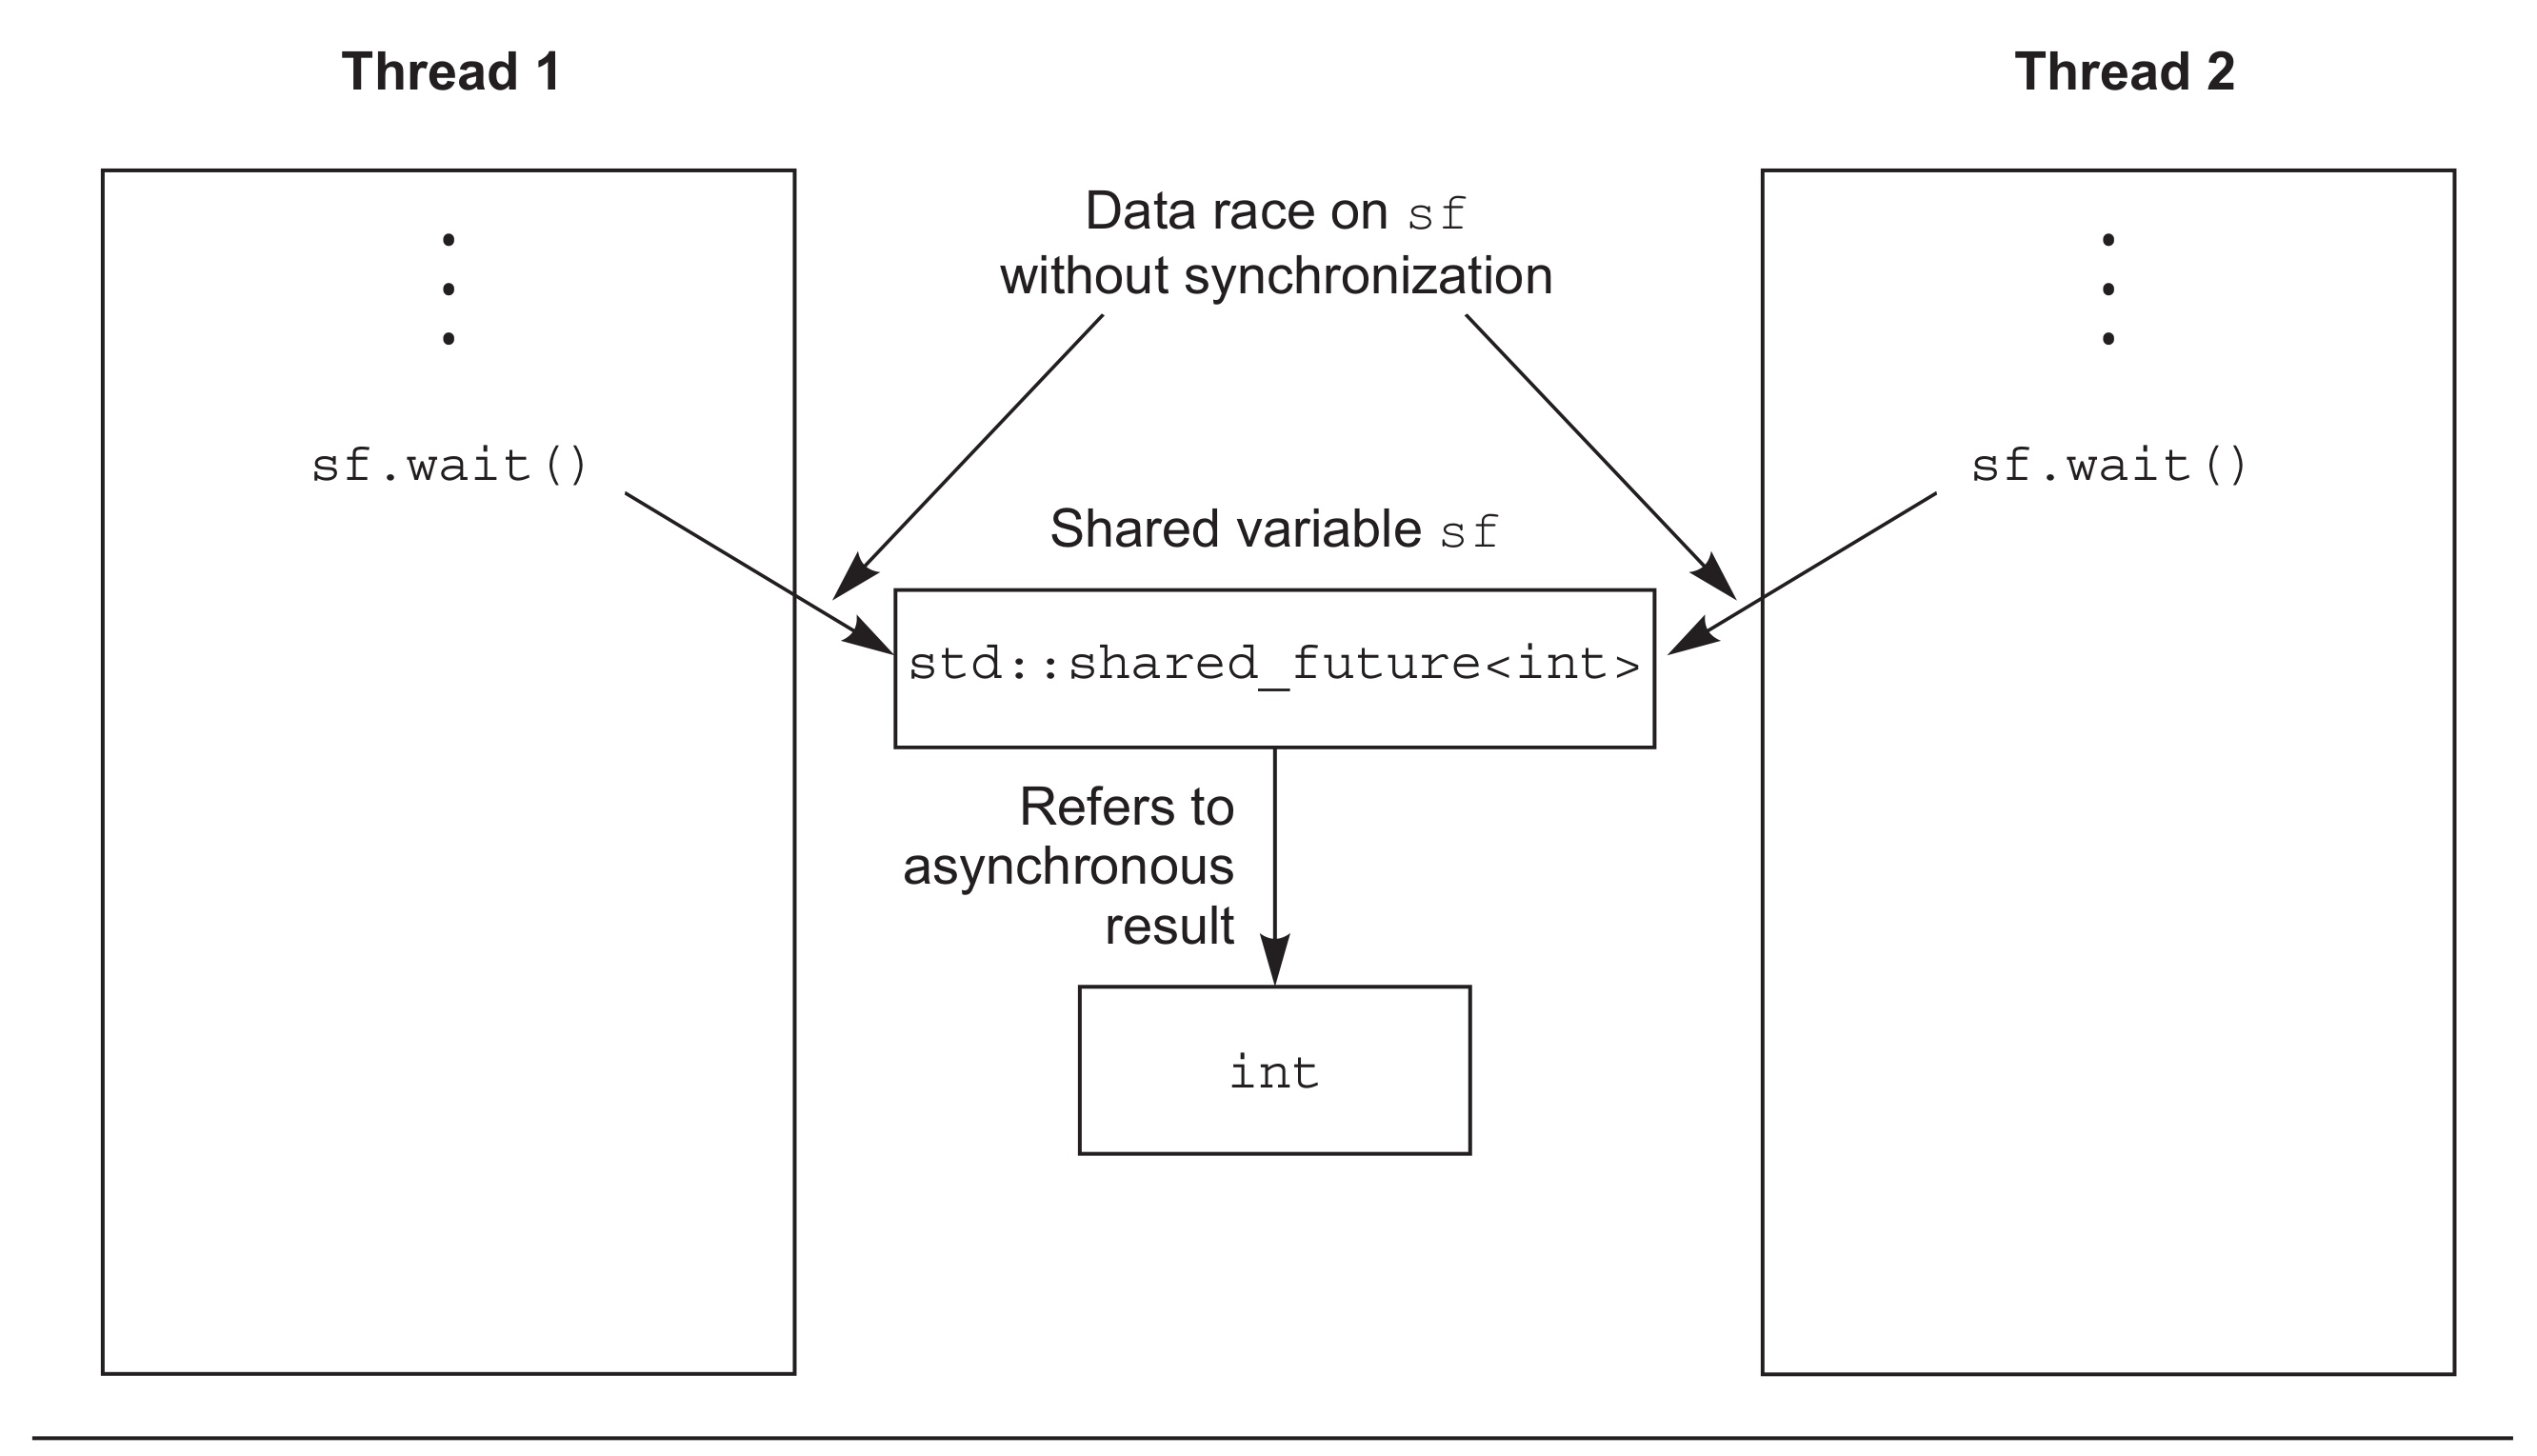
\includegraphics[width=0.7\textwidth]{content/chapter04/images/4-1-1.png}\\
  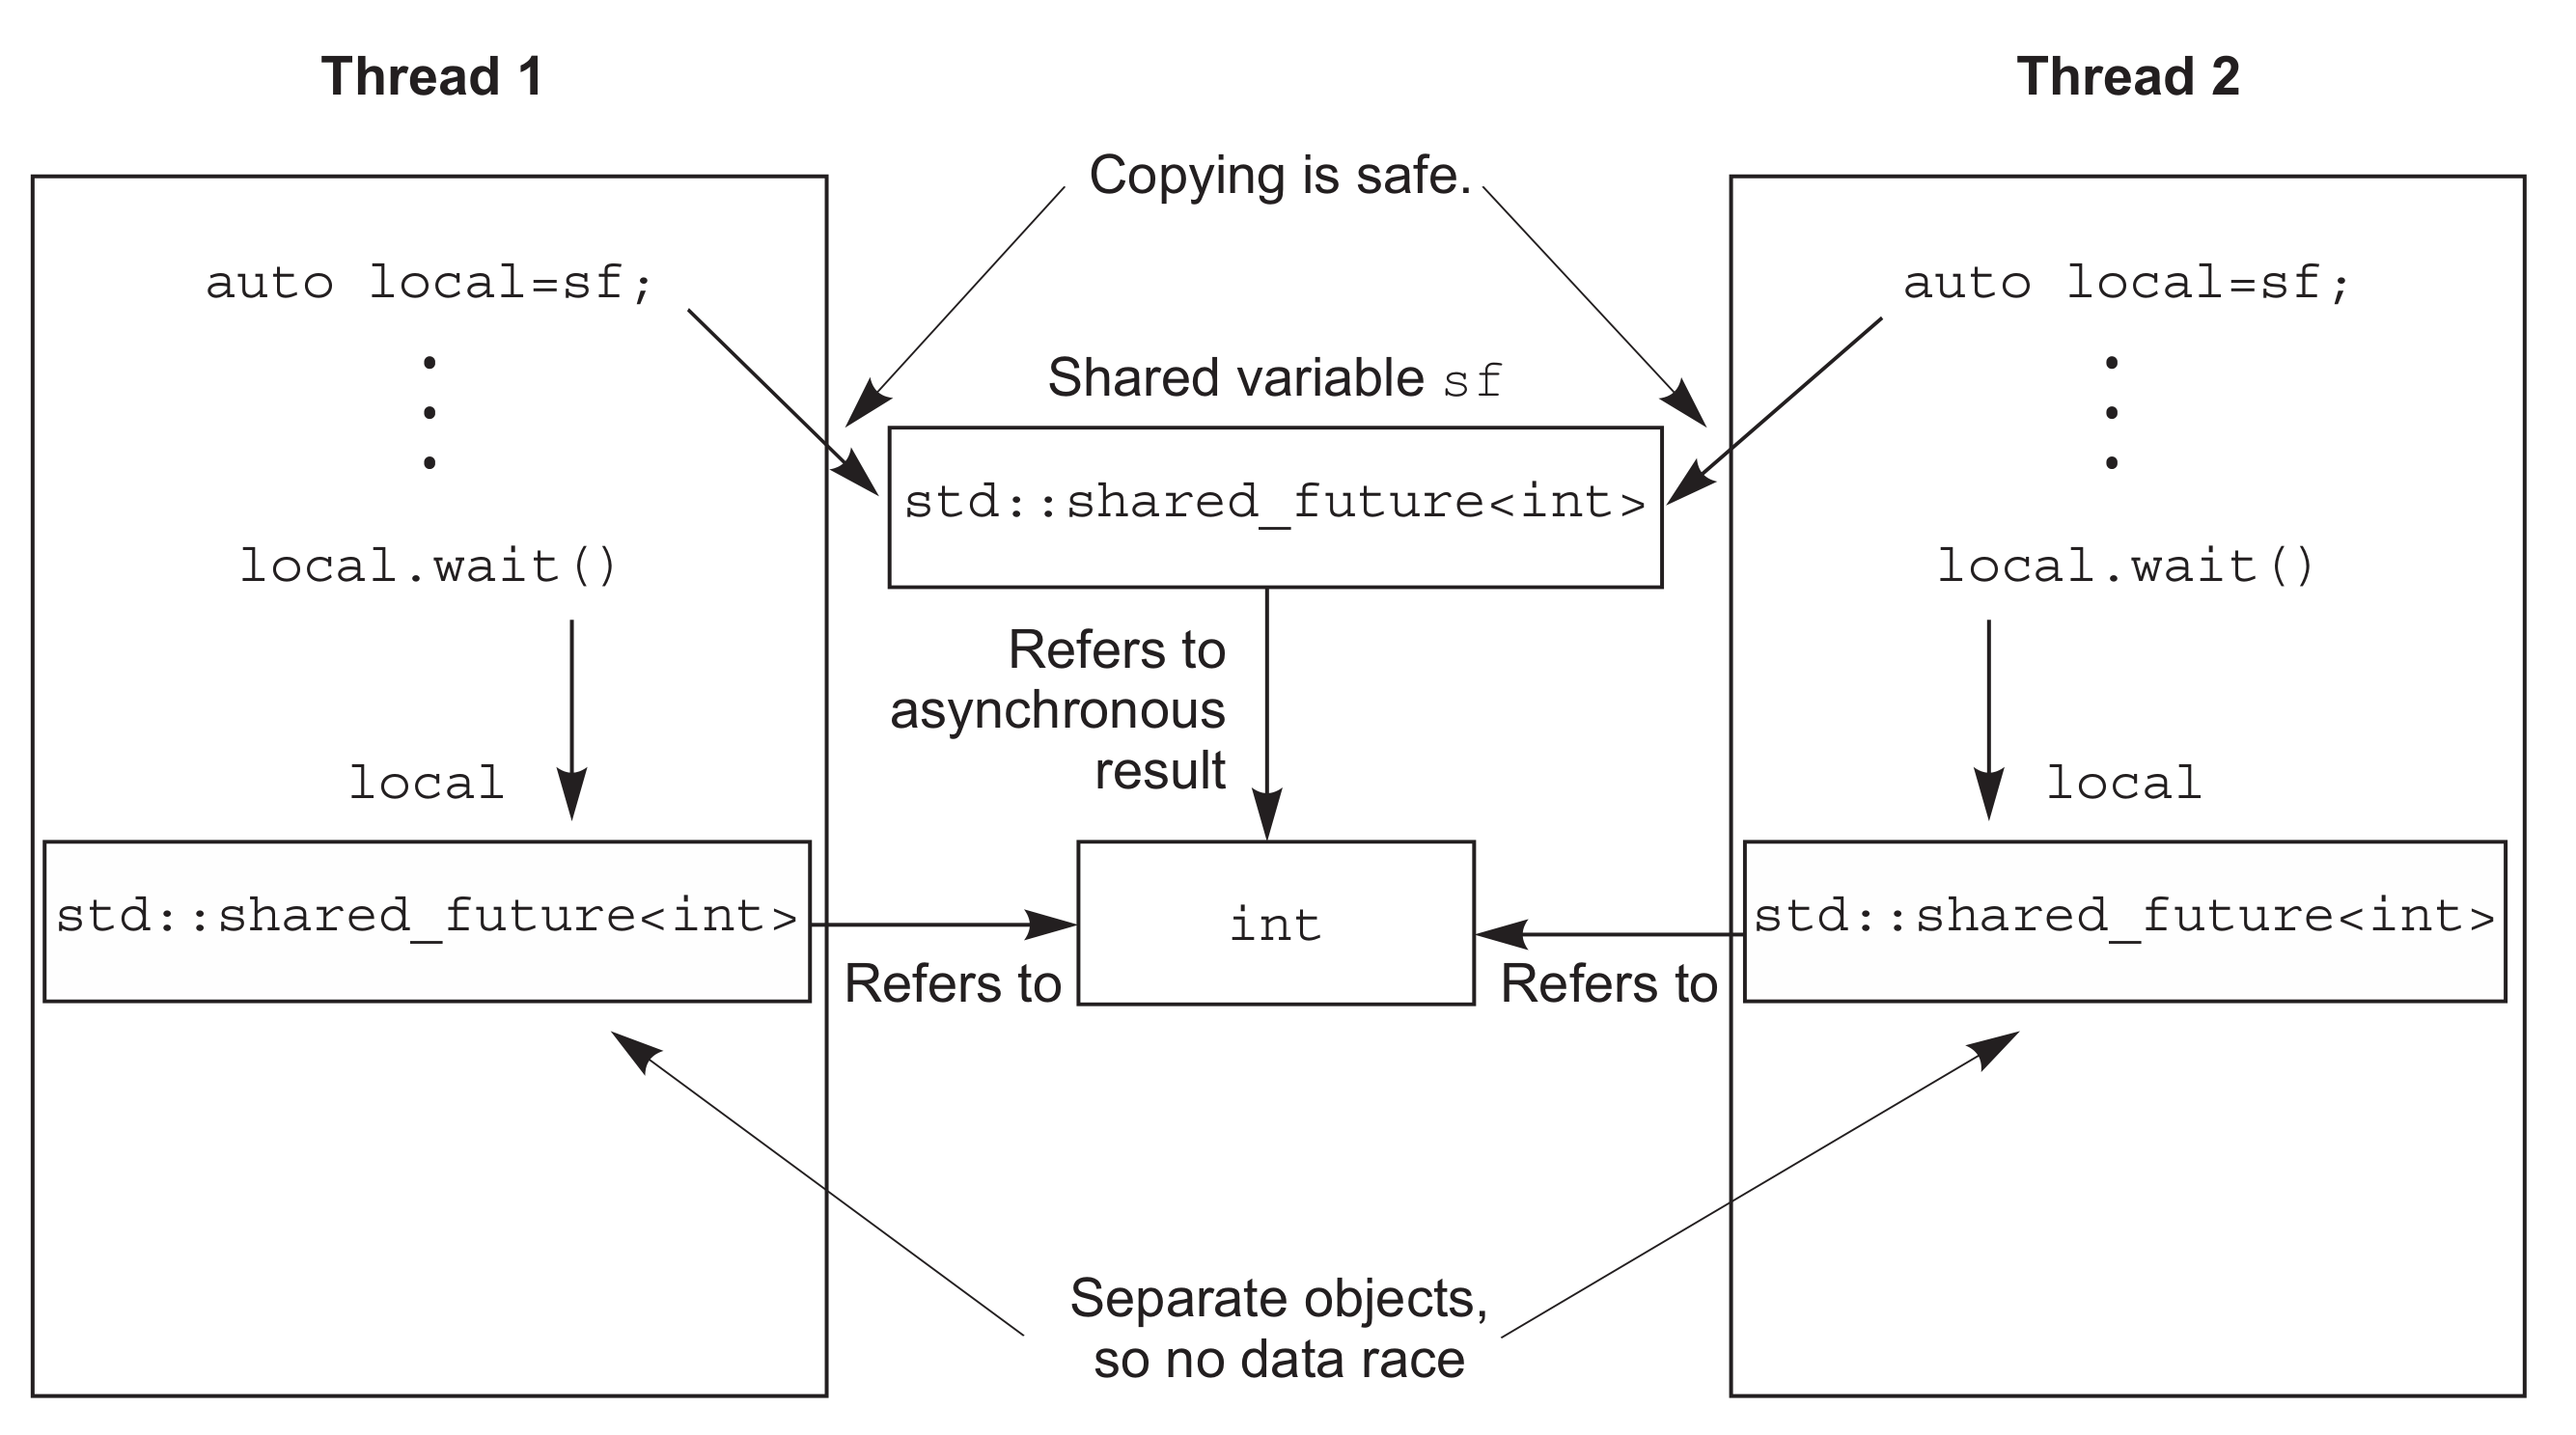
\includegraphics[width=0.7\textwidth]{content/chapter04/images/4-1-2.png}\\
  图4.1 使用多个\texttt{std::shared\_future}对象来避免数据竞争
\end{center}

可能会使用\texttt{std::shared\_future}的场景,例如:实现类似于复杂的电子表格的并行执行,每一个单元格有唯一终值,这个终值可能由其他单元格中的数据通过公式计算得到。公式计算得到的结果依赖于其他单元格,然后可以使用\texttt{std::shared\_future}对象引用第一个单元格的数据。当每个单元格内的所有公式并行执行后,任务会以期望的方式完成工作。不过,当其中有计算需要依赖其他单元格的值时就会阻塞,直到依赖单元格的数据准备就绪。这可以让系统在最大程度上使用硬件并发。

\texttt{std::shared\_future}的实例同步\texttt{std::future}实例的状态。当\texttt{std::future}对象没有与其他对象共享同步状态所有权,那么所有权必须使用\texttt{std::move}将所有权传递到\texttt{std::shared\_future},其默认构造函数如下:

\begin{cpp}
std::promise<int> p;
std::future<int> f(p.get_future());
assert(f.valid());  // 1 期望值 f 是合法的
std::shared_future<int> sf(std::move(f));
assert(!f.valid());  // 2 期望值 f 现在是不合法的
assert(sf.valid());  // 3 sf 现在是合法的
\end{cpp}

期望值f开始是合法的\symbol{"2460},因为引用的是promise p的同步状态,但是在转移sf的状态后,f就不合法了\symbol{"2461},而sf就是合法的了\symbol{"2462}。

如其他可移动对象一样,转移所有权是对右值的隐式操作,所以可以通过\texttt{std::promise}对象的成员函数get\_future()的返回值,直接构造一个\texttt{std::shared\_future}对象,例如:

\begin{cpp}
std::promise<std::string> p;
std::shared_future<std::string> sf(p.get_future());  // 1 隐式转移所有权
\end{cpp}

转移所有权是隐式的,用右值构造\texttt{std::shared\_future<>},得到\texttt{std::future<std::string>}类型的实例\symbol{"2460}。

\texttt{std::future}的这种特性,可促进\texttt{std::shared\_future}的使用,容器可以自动的对类型进行推断,从而初始化该类型的变量(详见附录A,A.6节)。\texttt{std::future}有一个share()成员函数,可用来创建新的\texttt{std::shared\_future} ,并且可以直接转移future的所有权。这样也就能保存很多类型,并且使得代码易于修改:

\begin{cpp}
std::promise< std::map< SomeIndexType, SomeDataType, SomeComparator,
     SomeAllocator>::iterator> p;
auto sf=p.get_future().share();
\end{cpp}

这个例子中,sf的类型推导为\texttt{std::shared\_future<std::map<SomeIndexType, SomeDataType, SomeComparator, SomeAllocator>::iterator>},还真的长。当比较器或分配器有所改动,只需要对promise的类型进行修改即可。future的类型会自动与promise的修改进行匹配。

有时需要限定等待事件的时间,不论是因为时间上有硬性规定(一段指定的代码需要在某段时间内完成),还是因为在事件没有很快的触发,或是有工作需要特定线程来完成,为了处理这种情况,需要等待函数能对超时进行指定。

